\ifx\wholebook\relax \else
% ------------------------ 

\documentclass{article}
%------------------- Other types of document example ------------------------
%
%\documentclass[twocolumn]{IEEEtran-new}
%\documentclass[12pt,twoside,draft]{IEEEtran}
%\documentstyle[9pt,twocolumn,technote,twoside]{IEEEtran}
%
%-----------------------------------------------------------------------------
%%
% loading packages
%
\newif\ifpdf
\ifx\pdfoutput\undefined % We're not running pdftex
  \pdffalse
\else
  \pdftrue
\fi
%
%
\ifpdf
  \RequirePackage[pdftex,%
            CJKbookmarks,%
       bookmarksnumbered,%
              colorlinks,%
          linkcolor=blue,%
              hyperindex,%
        plainpages=false,%
       pdfstartview=FitH]{hyperref}
\else
  \RequirePackage[dvipdfm,%
             CJKbookmarks,%
        bookmarksnumbered,%
               colorlinks,%
           linkcolor=blue,%
               hyperindex,%
         plainpages=false,%
        pdfstartview=FitH]{hyperref}
  \AtBeginDvi{\special{pdf:tounicode GBK-EUC-UCS2}} % GBK -> Unicode
\fi
\usepackage{hyperref}

% other packages
%-----------------------------------------------------------------------------
\usepackage{graphicx, color}
\usepackage{CJK}
%
% for programming 
%
\usepackage{verbatim}
\usepackage{listings}


\lstdefinelanguage{Smalltalk}{
  morekeywords={self,super,true,false,nil,thisContext}, % This is overkill
  morestring=[d]',
  morecomment=[s]{"}{"},
  alsoletter={\#:},
  escapechar={!},
  literate=
    {BANG}{!}1
    {UNDERSCORE}{\_}1
    {\\st}{Smalltalk}9 % convenience -- in case \st occurs in code
    % {'}{{\textquotesingle}}1 % replaced by upquote=true in \lstset
    {_}{{$\leftarrow$}}1
    {>>>}{{\sep}}1
    {^}{{$\uparrow$}}1
    {~}{{$\sim$}}1
    {-}{{\sf -\hspace{-0.13em}-}}1  % the goal is to make - the same width as +
    %{+}{\raisebox{0.08ex}{+}}1		% and to raise + off the baseline to match -
    {-->}{{\quad$\longrightarrow$\quad}}3
	, % Don't forget the comma at the end!
  tabsize=2
}[keywords,comments,strings]

\lstloadlanguages{C++, Lisp, Smalltalk}

% ======================================================================

\def\BibTeX{{\rm B\kern-.05em{\sc i\kern-.025em b}\kern-.08em
    T\kern-.1667em\lower.7ex\hbox{E}\kern-.125emX}}

\newtheorem{theorem}{Theorem}

%
% mathematics
%
\newcommand{\be}{\begin{equation}}
\newcommand{\ee}{\end{equation}}
\newcommand{\bmat}[1]{\left( \begin{array}{#1} }
\newcommand{\emat}{\end{array} \right) }
\newcommand{\VEC}[1]{\mbox{\boldmath $#1$}}

% numbered equation array
\newcommand{\bea}{\begin{eqnarray}}
\newcommand{\eea}{\end{eqnarray}}

% equation array not numbered
\newcommand{\bean}{\begin{eqnarray*}}
\newcommand{\eean}{\end{eqnarray*}}

\RequirePackage{CJK,CJKnumb,CJKulem,CJKpunct}
% we use CJK as default environment
\AtBeginDocument{\begin{CJK*}{GBK}{song}\CJKtilde\CJKindent\CJKcaption{GB}}
\AtEndDocument{\clearpage\end{CJK*}}

%
% loading packages
%
\newif\ifpdf
\ifx\pdfoutput\undefined % We're not running pdftex
  \pdffalse
\else
  \pdftrue
\fi
%
%
\ifpdf
  \RequirePackage[pdftex,%
       bookmarksnumbered,%
              colorlinks,%
          linkcolor=blue,%
              hyperindex,%
        plainpages=false,%
       pdfstartview=FitH]{hyperref}
\else
  \RequirePackage[dvipdfm,%
        bookmarksnumbered,%
               colorlinks,%
           linkcolor=blue,%
               hyperindex,%
         plainpages=false,%
        pdfstartview=FitH]{hyperref}
\fi
\usepackage{hyperref}

% other packages
%-----------------------------------------------------------------------------
\usepackage{graphicx, color}
%
% for programming 
%
\usepackage{verbatim}
\usepackage{listings}
\usepackage{algorithmic} %for pseudocode
\usepackage{algorithm}


\lstdefinelanguage{Smalltalk}{
  morekeywords={self,super,true,false,nil,thisContext}, % This is overkill
  morestring=[d]',
  morecomment=[s]{"}{"},
  alsoletter={\#:},
  escapechar={!},
  literate=
    {BANG}{!}1
    {UNDERSCORE}{\_}1
    {\\st}{Smalltalk}9 % convenience -- in case \st occurs in code
    % {'}{{\textquotesingle}}1 % replaced by upquote=true in \lstset
    {_}{{$\leftarrow$}}1
    {>>>}{{\sep}}1
    {^}{{$\uparrow$}}1
    {~}{{$\sim$}}1
    {-}{{\sf -\hspace{-0.13em}-}}1  % the goal is to make - the same width as +
    %{+}{\raisebox{0.08ex}{+}}1		% and to raise + off the baseline to match -
    {-->}{{\quad$\longrightarrow$\quad}}3
	, % Don't forget the comma at the end!
  tabsize=2
}[keywords,comments,strings]

\lstloadlanguages{C++, Lisp, Haskell, Python, Smalltalk}

% ======================================================================

\def\BibTeX{{\rm B\kern-.05em{\sc i\kern-.025em b}\kern-.08em
    T\kern-.1667em\lower.7ex\hbox{E}\kern-.125emX}}

\newtheorem{theorem}{Theorem}

%
% mathematics
%
\newcommand{\be}{\begin{equation}}
\newcommand{\ee}{\end{equation}}
\newcommand{\bmat}[1]{\left( \begin{array}{#1} }
\newcommand{\emat}{\end{array} \right) }
\newcommand{\VEC}[1]{\mbox{\boldmath $#1$}}

% numbered equation array
\newcommand{\bea}{\begin{eqnarray}}
\newcommand{\eea}{\end{eqnarray}}

% equation array not numbered
\newcommand{\bean}{\begin{eqnarray*}}
\newcommand{\eean}{\end{eqnarray*}}




\setcounter{page}{1}

\begin{document}

\fi
%--------------------------

% ================================================================
%                 COVER PAGE
% ================================================================

\title{Comparision of imperactive and functional implementation of binary search tree}

\author{Liu~Xinyu
\thanks{{\bfseries Liu Xinyu } \newline
  Email: liuxinyu95@gmail.com \newline
  Tel:   +86-1305-196-8666 \newline}
  }

\markboth{Binary search tree}
{imperactive and functional implementation}

\maketitle

\ifx\wholebook\relax
\chapter{Comparision of imperactive and functional implementation of binary search tree}

\section{abstruct}
\else
\begin{abstract}
\fi
This post list the imperactive and functional implementation of binary search tree. There are
multiple programming languages used, including, C++, Haskell, python and scheme/lisp (on going).
C++ and python are mostly used to show the imperactive implementation, while Haskell and Scheme are
used for functional purpose.

It's hard to say if imperactive is better than functional and vice versa, especially in binary search
tree case. Some times functional approach is much expressive (ex. in order walk), while in other case, 
imperactive one shows more merit factors (ex. to find successor and predeccesor).

There may be mistakes in the post, please feel free to point out.

This post is generated by \LaTeXe, and provided with GNU FDL(GNU Free Documentation License).
Please refer to http://www.gnu.org/copyleft/fdl.html for detail.

\ifx\wholebook\relax\else
\end{abstract}
\fi

\vspace{3cm}
{\bfseries Keywords:} Binary search tree, imperactive, functional, C++, Haskell, Python, Scheme/Lisp

{\bfseries Corresponding Author:} Liu Xinyu

\maketitle

% ================================================================
%                 Introduction
% ================================================================
\section{Introduction}
\label{introduction}

The concept of Binary tree itself is a recursive definition. Binary search tree is just a special type of
binary tree. The Binary tree is typically defined as below:

A binary tree is 
\begin{itemize}
\item either an empty node;
\item or a node contains 3 parts, a value, a left child which is a binary tree and a right child which is also a binary tree.
\end{itemize}

A binary search tree is a binary tree which satisfies the below criteria:
for each node in binary search tree,
\begin{itemize}
\item all the values in left child tree is less than the value of of this node;
\item the value of this node is less than any values in its right child tree.
\end{itemize}

This article provides implementation of binary search tree in C++, Haskell, Python, 
Scheme/Lisp languages. Including the definition, basic operation, such as
in-order walk, search, find min/max element, find successor/predecessor, insertion
and deletion. Most algorithms confirms to CLRS\cite{CLRS}.

All completed source code can be downloaded in appendix, please refer to appendix
for detailed information about build and run.

% ================================================================
% Definition
% ================================================================
\section{Definition}
\label{definition}

Based on the recursive definition of binary search tree, both imperactive and functinal 
languanges have very similar realization.

\subsubsection*{C++ definition. (mixed)}
\lstset{language=C++}
\begin{lstlisting}
template<class T>
struct node{
  node(T x):value(x), left(0), right(0), parent(0){}
  ~node(){ // for convinient, use functional approach
    if(left)
      delete left;
    if(right)
      delete right;
  }

  node* left; 
  node* right;
  node* parent; //parent is optional, it's helpful for succ/pred
  T value;
};
\end{lstlisting}

C++ definition of binary search tree is a struct, left
and right members can represent the children, the parent member is optional, but
it is helpful for implementation of succ/pred operation.

I used recursive approach in dtor to release the tree, this is just for 
convinience. I also provide a constructor (ctor) which can create a leaf
node easily.

\subsubsection*{Haskell definition. (functional)}
\lstset{language=Haskell}
\begin{lstlisting}
data Tree a = Empty 
            | Node (Tree a) a (Tree a) deriving (Show)
\end{lstlisting}

In C++, null pointer, which is 0 in ISO C++, is used to represent for empty
tree, while in Haskell, an explicit constructor Empty is used. The derivation
of Show is just for easy printing the result.

% ================================================================
% Helper functions
% ================================================================
\subsection{Helper functions}

Besides the functions which are mentioned in CLRS\cite{CLRS}. I provided some
extra helper functions. They typically helps do some common works such as 
access element of a tree, creation leaf and release memory.

\subsubsection{common helper functions}

\subsubsection*{C++ helper function.}
\lstset{language=C++}
\begin{lstlisting}
// cut the node off the tree, then delete it.
// it can prevent dtor removed children of a node
template<class T>
void remove_node(node<T>* x){
  if(x)
    x->left = x->right = 0;
  delete x;
}
\end{lstlisting}

The remove\_node() function can only release memory of a single node without recursively
removing all its children. 

\begin{lstlisting}
template<class T>
std::string tree_to_str(const node<T>* tree){
  if(tree){
    std::ostringstream s;
    s<<"("<<tree_to_str(tree->left)<<"), "<<tree->value
     <<", ("<<tree_to_str(tree->right)<<")";
    return s.str();
  }
  return "empty";
}

template<class T>
node<T>* clone_tree(const node<T>* t, node<T>* parent=0){
  if(t){
    node<T>* t1 = new node<T>(t->value);
    t1->left = clone_tree(t->left, t1);
    t1->right = clone_tree(t->right, t1);
    t1->parent = parent;
    return t1;
  }
  return static_cast<node<T>*>(0);
}
\end{lstlisting}

The tree\_to\_str() function can generate a string
to represent the tree data. For empty data, it just prints (empty); in other case
it prints (...left..., key, ...right...). This function is implemented in a
functional way.

The function clone\_tree() provides a way to duplicate a exist tree. This
function is realized in a recursive manner.

\subsubsection*{Haskell helper functions. (pattern-matching)}
\lstset{language=Haskell}
\begin{lstlisting}
leaf::a -> Tree a
leaf a = Node Empty a Empty

left::Tree a -> Tree a
left (Node l _ _) = l
left _ = Empty

right::Tree a -> Tree a
right (Node _ _ r) = r
right _ = Empty

key::Tree a -> a
key (Node _ k _) = k

isEmpty::Tree a -> Bool
isEmpty Empty = True
isEmpty _ = False
\end{lstlisting}

leaf function can create a leaf node with specified value; left and right
are used to get the left sub tree and right sub tree. key function is
used to return the value of a node. isEmpty function can test if a node
is an empty node.

\subsubsection{collection to tree helper function}
It is convenient to have a function which can turn a collection, such as
an array, a list etc into a tree. The generation process has to call insertion
function which will be defined in later section.

\subsubsection*{C++ collection to tree}
\lstset{language=C++}
\begin{lstlisting}
template<class Coll>
node<typename Coll::value_type>* 
build_tree(const Coll& coll){
  node<typename Coll::value_type>* tree(0);
  for(typename Coll::const_iterator it=coll.begin(); 
      it!=coll.end(); ++it)
    tree = insert(tree, *it);
  return tree;
}
\end{lstlisting}

The function build\_tree() can create a tree object from a STL collection 
by calling insert(). insert() will be defined in later section. this function
is written in a imperactive way.

\subsubsection*{Haskell list to tree}
\lstset{language=Haskell}
\begin{lstlisting}
listToTree::(Ord a)=>[a] -> Tree a
listToTree lst = foldl (\t x -> insert t x) Empty lst
\end{lstlisting}

This function is implemented in a functional way by using foldl.

To test if the function works porperly, we can use the below test code.
\subsubsection*{C++ test for build tree}
\lstset{language=C++}
\begin{lstlisting}
const int buf[]={15, 6, 18, 3, 7, 17, 20, 2, 4, 13, 9};
tree = build_tree(std::vector<int>(buf, 
         buf+sizeof(buf)/sizeof(int)));
std::cout<<tree_to_str(tree);
\end{lstlisting}

This program will output:
\begin{verbatim}
((((empty), 2, (empty)), 3, ((empty), 4, (empty))), 6, ((empty), 
7, (((empty), 9, (empty)), 13, (empty)))), 15, (((empty), 17, 
(empty)), 18, ((empty), 20, (empty)))
\end{verbatim}

\subsubsection*{Haskell test for listToTree}
\lstset{language=Haskell}
\begin{lstlisting}
t2 = listToTree [15, 6, 18, 3, 7, 17, 20, 2, 4, 13, 9]
putStrLn ("\ntest create from list:\t" ++ show t2)
\end{lstlisting}

This program will output:
\begin{verbatim}
test create from list:  Node (Node (Node (Node Empty 2 Empty) 3 
(Node Empty 4 Empty)) 6 (Node Empty 7 (Node (Node Empty 9 Empty) 
13 Empty))) 15 (Node (Node Empty 17 Empty) 18 (Node Empty 20 
Empty))
\end{verbatim}


% ================================================================
% In-order walk
% ================================================================
\subsection{In-order walk}

There are 3 ways to traverse a binary tree, preorder tree walk, inorder 
tree walk, and postorder tree walk; inorder tree walk is particularly helpful
for binary search tree, because it can access node in ordered value.

It's hard to write imperactive way of inorder tree walk, so I only provide
functional implementation. It is expressive.

Inorder tree walk can be described as the following:
\begin{itemize}
\item If the tree is empty, just return;
\item traverse the left child by inorder walk, then access the key, 
finally traverse the right child by inorder walk.
\end{itemize}

\subsubsection*{C++ in-order walk. (functional)}
\lstset{language=C++}
\begin{lstlisting}
// easy implemented by using functional approach
template<class T, class F>
void in_order_walk(node<T>* t, F f){
  if(t){
    in_order_walk(t->left, f);
    f(t->value);
    in_order_walk(t->right, f);
  }
}
\end{lstlisting}

The function takes a parameter f, it can be a real function, or a function
object, this program will apply f to the node by inorder tree walk.

\subsubsection*{Haskell in-order walk. (functional)}
\lstset{language=Haskell}
\begin{lstlisting}
inOrderWalk::Tree a -> (a->b) -> Tree b
inOrderWalk Empty f = Empty
inOrderWalk t f = (Node (inOrderWalk (left t) f) 
            (f (key t)) (inOrderWalk (right t) f))
\end{lstlisting}

To test the result of this function, we need creat a tree first. Insertion
must be provided for tree creation, please refer to later sections for the
details of how to create a tree. I'll use the result directly here.

In this article, I'll use an example tree as in figure \ref{fig:example-tree}.

\begin{figure}[htbp]
       \begin{center}
	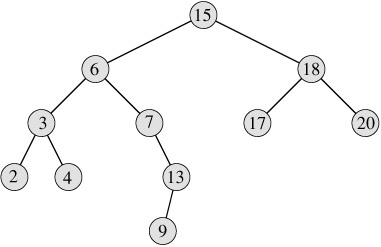
\includegraphics[scale=0.5]{img/tree.eps}
        \caption{example tree} \label{fig:example-tree}
       \end{center}
\end{figure}

\subsubsection*{C++ in-order walk testing and it's result.}

Suppose we have a pointer point to the tree contains data in figure 
\ref{fig:example-tree}. It can be created by build\_tree() function.

\lstset{language=C++}
\begin{lstlisting}
  struct Print{
    template<class T>
    void operator()(T x){ std::cout<<x<<", "; }
  };

  //...
  std::cout<<"test in order walk with print functor: ";
  in_order_walk(tree, Print());
\end{lstlisting}

In the above example, I created a function object Print, and pass an
instance of it to in-order walk process, it will print all the node
from less to greater with ',' as deliminator.

\begin{verbatim}
test in order walk with print functor: 2, 3, 4, 6, 7, 9, 13, 15, 
17, 18, 20,
\end{verbatim}

While the Haskell version can be tested as below:

\lstset{language=Haskell}
\begin{lstlisting}
testTreeWalk = "test tree in-order walk by apply (-):\t"++
               show (inOrderWalk t2 (\x -> -x))
putStrLn testTreeWalk
\end{lstlisting}

It will output:
\begin{verbatim}
test tree in-order walk by apply (-):   Node (Node (Node 
(Node Empty (-2) Empty) (-3) (Node Empty (-4) Empty)) (-6) 
(Node Empty (-7) (Node (Node Empty (-9) Empty) (-13) 
Empty))) (-15) (Node (Node Empty (-17) Empty) (-18) (Node 
Empty (-20) Empty))
\end{verbatim}

% ================================================================
% Querying a binary search tree
% ================================================================
\section{Querying a binary search tree}

This section provides implementation of querying operations which are
described in 12.2 of CLRS\cite{CLRS}

\subsection{Searching}
In CLRS\cite{CLRS}, searching is demonstrated in both recursive way and 
imperactive way. According to the definition of binary search tree, search
a value in a tree can be realized in the following recursive manner.

\begin{itemize}
\item If the tree is empty, just return empty (not-found);
\item If the key of the root is equal to the value to be found, 
return the root;
\item If the value is less than the key of the root, search in the left
child.
\item Else, which means that the value is greater than the key of the 
root, search in the right child.
\end{itemize}

\subsubsection*{Haskell search implementation, functional}
\lstset{language=Haskell}
\begin{lstlisting}
search::(Ord a)=> Tree a -> a -> Tree a
search Empty _ = Empty
search t x | key(t)==x = t
           | x < key(t) = search (left t) x
           | otherwise = search (right t) x
\end{lstlisting}

Hakell program of search is just translate the above recursive algorithm
description into code. Since it uses less than operator '<', the type
of the key value must be comparable. So the type variable is an instance 
of Ord type class.

\subsubsection*{C++ search implementation, imperactive}
\lstset{language=C++}
\begin{lstlisting}
template<class T>
node<T>* search(node<T>* t, T x){
  while(t && t->value!=x){
    if(x < t->value) t=t->left;
    else t=t->right;
  }
  return t;
}
\end{lstlisting}

Search can also be implemented in an imperactive way by replace the current
node to left child if the value to be search less than the key or to right 
child if greater than.

\subsection{Minimun and maximum}

to do ...

\subsection{Successor and predecessor}

to do ...

% ================================================================
%                 Insertion and deletion
% ================================================================
\section{Insertion and deletion}

to do...

\subsection{Insertion}

to do ...

\subsection{Deletion}

to do ...

\section{Appendix}
%\appendix
download position: http://liuxinyu95.googlepages.com/particlesys.cpp
appendix to do ...

\begin{thebibliography}{99}

\bibitem{CLRS}
Thomas H. Cormen, Charles E. Leiserson, Ronald L. Rivest and Clifford Stein. 
``Introduction to Algorithms, Second Edition''. ISBN:0262032937. The MIT Press. 2001

\bibitem{kedama}
Oshima Yoshiki. Kedama: A massively-parallel tile-scriptable particle system. http://www.is.titech.ac.jp/~ohshima/squeak/kedama/

\end{thebibliography}

\ifx\wholebook\relax\else
\end{document}
\fi
